\section{Auswertung}

Die in der Auswertung bestimmten Ausgleichsrechnungen werden mit
der Funktion \emph{curve\_ fit} aus dem Python Paket \emph{scipy.optimize}\cite{scipy} durchgeführt. %cite nach paket reicht

\subsection{Auswertung der $T_{00}$ Mode}
\FloatBarrier
In der Tabelle \ref{tab: T_00} befinden sich die aufgenommenen Messwerte.
\begin{table} 
\centering 
\caption{Messwerte der T_00 Mode.} 
\label{tab: T_00} 
\begin{tabular}{S S } 
\toprule  
{$r / \si{ \milli\meter }$} & {$I_p / \si{ \micrompere}$} \\ 
\midrule  
-10.0 & 2.2\\ 
-9.0 & 3.1\\ 
-8.0 & 3.9\\ 
-7.0 & 5.0\\ 
-6.0 & 6.2\\ 
-5.0 & 7.4\\ 
-4.0 & 8.4\\ 
-3.0 & 9.4\\ 
-2.0 & 9.4\\ 
-1.0 & 9.2\\ 
0.0 & 8.8\\ 
1.0 & 8.1\\ 
2.0 & 7.2\\ 
3.0 & 6.1\\ 
4.0 & 5.0\\ 
5.0 & 3.8\\ 
6.0 & 2.7\\ 
7.0 & 1.9\\ 
8.0 & 1.2\\ 
9.0 & 0.7\\ 
10.0 & 0.4\\ 
\bottomrule 
\end{tabular} 
\end{table}
Weiterhin werden die Messdaten in Abbildung \ref{fig: T_00} grafisch dargestellt.
\begin{figure}[h!]
  \centering
  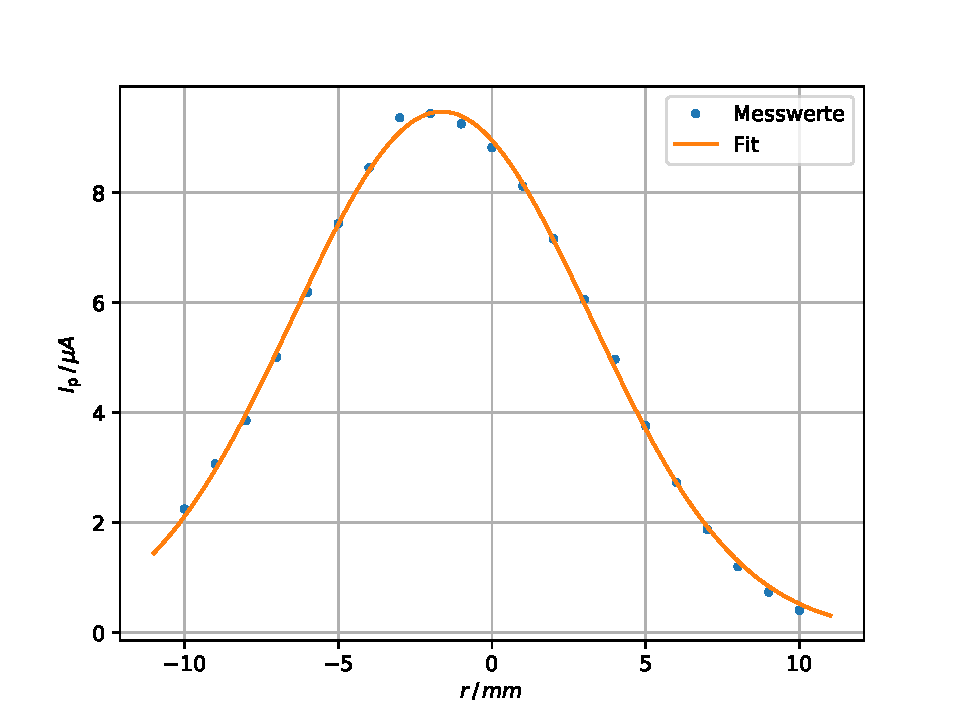
\includegraphics[width=0.7\textwidth]{../Messdaten/plots/T_00.pdf}
  \caption{Plot der in Tabelle \ref{tab: T_00} gelisteten Messwerte. Zusätzlich ist in der Grafik die bestimmte Ausgleichskurve zu sehen.}
  \label{fig: T_00}
\end{figure}
In der Abbildung ist die mit Hilfe von \emph{scipy.optimize} erstelle Fit an die Funktion \eqref{eq: tem00} zu erkennen. %eqref
Aus der Ausgleichsrechnung ergeben sich die folgenden Parameter

\begin{align}
  \label{eq: fit_t_00}
  \begin{aligned}
  I_0&=\SI{9.47 \pm 0.05}{\micro\ampere}\\
  d_0&=\SI{-1.63\pm 0.03}{\milli\meter}\\
  \omega&=\SI{9.67\pm0.06}{\per\milli\meter}
\end{aligned}
\end{align}
\FloatBarrier
\subsection{Auswertung der $T_{10}$ Mode}
\FloatBarrier
Die bei der Vermessung der $T_{10}$ Mode aufgenommen Messwerte sind in der Tabelle
\ref{tab: T_10} notiert.
\begin{table} 
\centering 
\caption{Messwerte der T_10 Mode.} 
\label{tab: T_10} 
\begin{tabular}{S S } 
\toprule  
{$r / \si{ \milli\meter }$} & {$I_p / \si{ \micrompere}$} \\ 
\midrule  
-10.0 & 0.2\\ 
-9.0 & 0.5\\ 
-8.0 & 0.8\\ 
-7.0 & 1.3\\ 
-6.0 & 1.6\\ 
-5.0 & 1.9\\ 
-4.0 & 2.0\\ 
-3.0 & 2.0\\ 
-2.0 & 1.5\\ 
-1.0 & 0.8\\ 
0.0 & 0.3\\ 
1.0 & 0.1\\ 
2.0 & 0.0\\ 
3.0 & 0.2\\ 
4.0 & 0.7\\ 
5.0 & 1.2\\ 
6.0 & 1.7\\ 
7.0 & 1.6\\ 
8.0 & 1.3\\ 
9.0 & 1.2\\ 
10.0 & 1.0\\ 
11.0 & 0.6\\ 
12.0 & 0.3\\ 
13.0 & 0.2\\ 
14.0 & 0.1\\ 
15.0 & 0.0\\ 
\bottomrule 
\end{tabular} 
\end{table}
An die Messwerte wird eine Funktion der Form \eqref{eq: tem01} gefittet, hierbei wird für %präsenz, eqref
die Funktion \emph{curve\_fit} die folgenden Startparameter gewählt
\begin{align*}
  I_{0,1}&=\SI{2.03}{\micro\ampere} & I_{0,2}&=\SI{1.68}{\micro\ampere}\\       %würde ich weglassen, wofür ist das relevant? % Ohne Startparameter funktioniert der Fit nicht, dient der Überprüfbarkeit
  d_{0,1}&=\SI{-4}{\milli\meter}& d_{0,2}&=\SI{6.0}{\milli\meter} \\
  \omega_1&=\SI{1}{\per\milli\meter} &   \omega_2&=\SI{1}{\per\milli\meter}.
\end{align*}
Das Ergebnis der Ausgleichsberechnung lautet
\begin{align}
  \label{eq: fit_t_10}
  \begin{aligned}
  I_{0,1}&=\SI{2.09\pm0.09}{\micro\ampere} & I_{0,2}&=\SI{1.66\pm0.09}{\micro\ampere}\\   %wieso nicht mit \SI{a(b)}?
  d_{0,1}&=\SI{-4.38\pm0.12}{\milli\meter}& d_{0,2}&=\SI{7.28\pm0.15}{\milli\meter} \\
  \omega_1&=\SI{4.99\pm0.24}{\per\milli\meter} &   \omega_2&=\SI{4.88\pm0.30}{\per\milli\meter}.
\end{aligned}
\end{align}
Die Regressionskurve und die Messdaten sind in Abbildung \ref{fig: T_10} dargestellt.
\begin{figure}[h!]
  \centering
  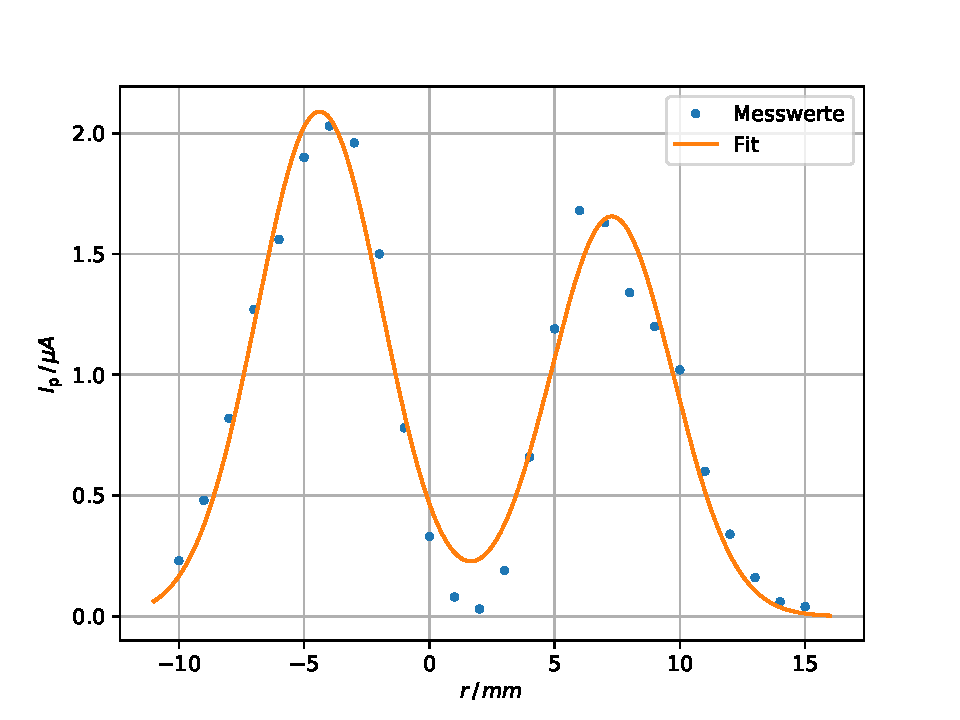
\includegraphics[width=0.8\textwidth]{../Messdaten/plots/T_10.pdf}
  \caption{Plot der in Tabelle \ref{tab: T_10} gelisteten Messwerte. Zusätzlich ist in der Grafik die bestimmte Ausgleichskurve zu sehen.}
  \label{fig: T_10}
\end{figure}
\FloatBarrier
\subsection{Auswertung der Polarisation}

In der Tabelle \ref{tab: pola} sind die notierten Werte der Polarisationsmessung
aufgelistet.
\FloatBarrier
\begin{table} 
\centering 
\caption{Aufgenommene Werte bei der Polarisationsmessungs.} 
\label{tab: pola} 
\begin{tabular}{S S S S S S S S S } 
\toprule  
{$\varphi / \si{ \degree }$} & {$\varphi / \si{ \radian }$} & {$I_p / \si{ \milli\ampere}$} & {$\varphi / \si{ \degree }$} & {$\varphi / \si{ \radian }$} & {$I_p / \si{ \milli\ampere}$} & {$\varphi / \si{ \degree }$} & {$\varphi / \si{ \radian }$} & {$I_p / \si{ \milli\ampere}$} \\ 
\midrule  
0 & 0.00 & 0.36 & 130 & 2.27 & 0.75 & 260 & 4.54 & 0.21\\ 
10 & 0.17 & 0.23 & 140 & 2.44 & 0.74 & 270 & 4.71 & 0.34\\ 
20 & 0.35 & 0.12 & 150 & 2.62 & 0.69 & 280 & 4.89 & 0.47\\ 
30 & 0.52 & 0.04 & 160 & 2.79 & 0.61 & 290 & 5.06 & 0.58\\ 
40 & 0.70 & 0.00 & 170 & 2.97 & 0.51 & 300 & 5.24 & 0.67\\ 
50 & 0.87 & 0.01 & 180 & 3.14 & 0.36 & 310 & 5.41 & 0.74\\ 
60 & 1.05 & 0.06 & 190 & 3.32 & 0.24 & 320 & 5.59 & 0.76\\ 
70 & 1.22 & 0.16 & 200 & 3.49 & 0.14 & 330 & 5.76 & 0.73\\ 
80 & 1.40 & 0.28 & 210 & 3.67 & 0.06 & 340 & 5.93 & 0.64\\ 
90 & 1.57 & 0.41 & 220 & 3.84 & 0.01 & 350 & 6.11 & 0.52\\ 
100 & 1.75 & 0.50 & 230 & 4.01 & 0.00 & 360 & 6.28 & 0.39\\ 
110 & 1.92 & 0.62 & 240 & 4.19 & 0.03 &  &  & \\ 
120 & 2.09 & 0.71 & 250 & 4.36 & 0.10 &  & & \\ 
\bottomrule 
\end{tabular} 
\end{table}
 %besser varphi
An die Messwerte wird die Funktion \eqref{eq: malus} %kannst du auch referenziere, habe ich in der theorie
mit den folgenden Parametern gefittet:

\begin{align}
  \label{eq: fit_pola}
  \begin{aligned}
  I_0&=\SI{0.748\pm0.005}{\milli\ampere}\\ %s.o.
  \phi_0&=\SI{0.792\pm0.006}{\radian}
\end{aligned}
\end{align}
Die Messwerte und die Ausgleichskurve sind in Abbildung \ref{fig: pola} skizziert.

\begin{figure}[h!]
  \centering
  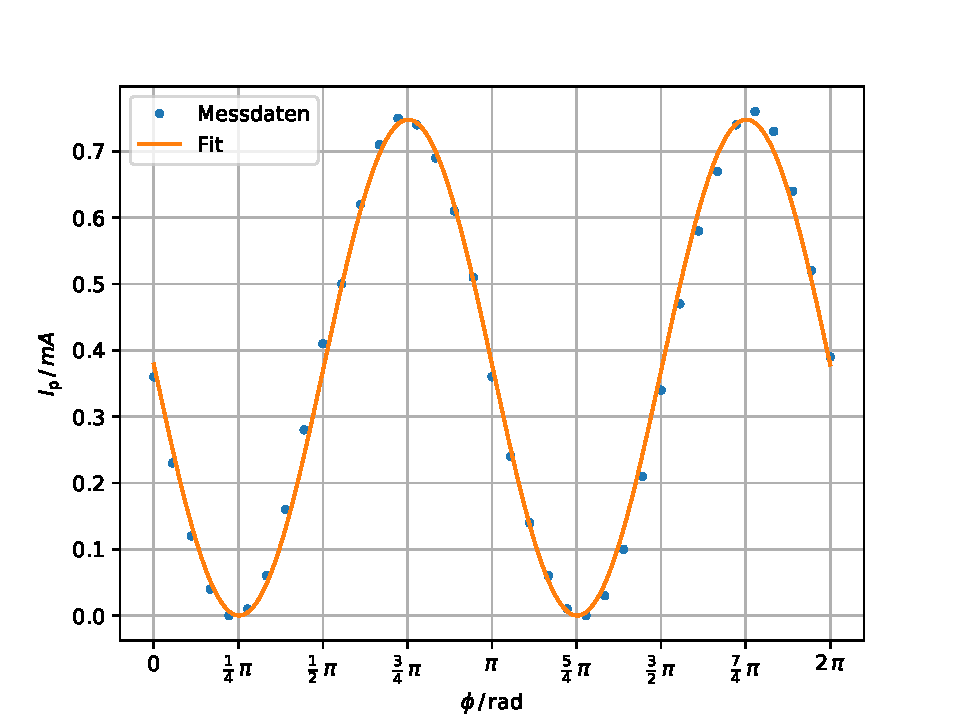
\includegraphics[width=0.8\textwidth]{../Messdaten/plots/pola.pdf}
  \caption{Plot der in Tabelle \ref{tab: pola} gelisteten Messwerte. Zusätzlich ist in der Grafik die bestimmte Ausgleichskurve zu sehen.}
  \label{fig: pola}
\end{figure}
\FloatBarrier

\FloatBarrier
\subsection{Wellenlängenbestimmung}
Die Messwerte, um die Wellenlänge des Lasers zu bestimmen, befinden sich in Tabelle  \ref{tab: wellenlaenge}.
Bei der Messung beträgt der Abstand zum Schirm $L=\SI{83}{\centi\meter}$ %präsenz
und wird mit einem Gitter mit dem Gitterabstand von $a=\SI{1e-5}{\meter}$ durchgeführt. %präsenz
\begin{table} 
\centering 
\caption{Aufgenommene Messwerte für die Wellenlängenbestimmung. Der Winkel $	\theta$ und die Wellenlänge $\lambda$ werden mit den Gleichung \eqref{} und \eqref{} bestimmt. Der Abstand zum Schirm beträgt $l=\SI{83}{\centi\meter}$ und der Gitterabstand $a=\SI{1e-5}{\meter}$.} 
\label{tab: wellenlaenge} 
\begin{tabular}{S S S S } 
\toprule  
{$n $} & {$d / \si{ \centi\meter}$} & {$\theta / \si{ \radian}$} & {$\lambda / \si{ \nano\meter}$} \\ 
\midrule  
1.0 & 10.8 & 0.1 & 649.2\\ 
2.0 & 21.6 & 0.1 & 645.2\\ 
3.0 & 32.7 & 0.2 & 644.2\\ 
4.0 & 44.0 & 0.3 & 640.5\\ 
5.0 & 51.2 & 0.3 & 589.5\\ 
6.0 & 70.0 & 0.4 & 647.6\\ 
\bottomrule 
\end{tabular} 
\end{table}

In der Tabelle werden außerdem die für jede Ordnung $n$ errechneten Wellenlängen $\lambda$ und Winkel $\theta$
mit aufgelistet. Hierbei wird für die Berechnung der Wellenlänge und des Winkels die Formel \eqref{eq: interferenz} verwendet. %eqref, winkelgleichung nicht explizit aufgeführt, kannst du hier nochmal hinschreiben
Über alle vermessenen Ordnungen gemittelt ergibt sich für die Wellenlänge
\begin{equation}
  \label{eq: mittelwert_wellenlaenge}
  \ov{\lambda}=\SI{636\pm9}{\nano\meter}.
\end{equation}
\FloatBarrier
\FloatBarrier
\subsection{Untersuchung der Stabilitätsbedingung} %Untersuchung
Die Stabilitätsbedingung wird für zwei verschiedene Konfigurationen untersucht,
zum anderen werden für den Resonator zwei konkave Spiegel verwendet und zum andern %anderen
ein konkaver und ein ebener Spiegel. %ebener
Um einen Vergleich zwischen den Messwerten und der Theorie zu ermöglichen, wird der gemessene
Photostrom $I_p$ wie folgt umkskaliert: %I
\begin{equation*}
  I_p \rightarrow \frac{I_p\cdot c}{I_{p,max}}.
\end{equation*}
Hierbei wird der Skalierungsfaktor $c$ aus Startlänge $d_0$ der jeweiligen Konfiguration (legt $r_i$ fest) und der Formel
\eqref{} berechnet. %eqref
\begin{equation*}
  c=g_1g_2(d_0, r_1, r_2)
\end{equation*}

\FloatBarrier
\FloatBarrier
\subsubsection{Konfokale Konfiguration} %oder konfokale

Die für diese Konfiguration aufgenommenen Messwerte befinden sich in Tabelle \ref{fig: konkon}.
\begin{table} 
\centering 
\caption{Aufgenommene Messwerte für die Untersuchung der Stabilitätsbedingung bei Konkav-Konkave Konfiguration. Der Umskalierungsfaktor $c$ beträgt $\num{0.12}$.} 
\label{tab: konkon} 
\begin{tabular}{S S S } 
\toprule  
{$ d / \si{ \centi\meter}$} & {$ I_p / \si{ \milli\ampere}$} & {$ \frac{I_p\cdot c}{I_{p,max}} $} \\ 
\midrule  
91 & 0.43 & 0.12\\ 
100 & 0.40 & 0.11\\ 
106 & 0.42 & 0.12\\ 
116 & 0.33 & 0.09\\ 
126 & 0.35 & 0.10\\ 
131 & 0.37 & 0.11\\ 
134 & 0.24 & 0.07\\ 
141 & 0.34 & 0.10\\ 
147 & 0.16 & 0.05\\ 
157 & 0.42 & 0.12\\ 
\bottomrule 
\end{tabular} 
\end{table}

Der Skalierungsfaktor trägt den Wert $c=\num{0.12}$.
An die skalierten Messwerte wird eine quadratische Funktion der Form
\begin{equation*}
  f(d)=a\,d^2+b\,d+c
\end{equation*}
gefittet. Aus der Ausgleichsrechnung folgen die Werte
\begin{align}
  \label{eq: fit_konkon}
  \begin{aligned}
    a&=\SI{2.0\pm 1.9 e-5}{\per\square\milli\meter}\\
    b&=\SI{-6\pm5 e-3}{\per\milli\meter}\\
    c&=\num{0.47\pm0.28}.
  \end{aligned}
\end{align}
In der Grafik \ref{fig: konkon} werden die Messwerte, der Fit und die Theoriekurve \eqref{} miteinander verglichen. %eqref

\begin{figure}[h!]
  \centering
  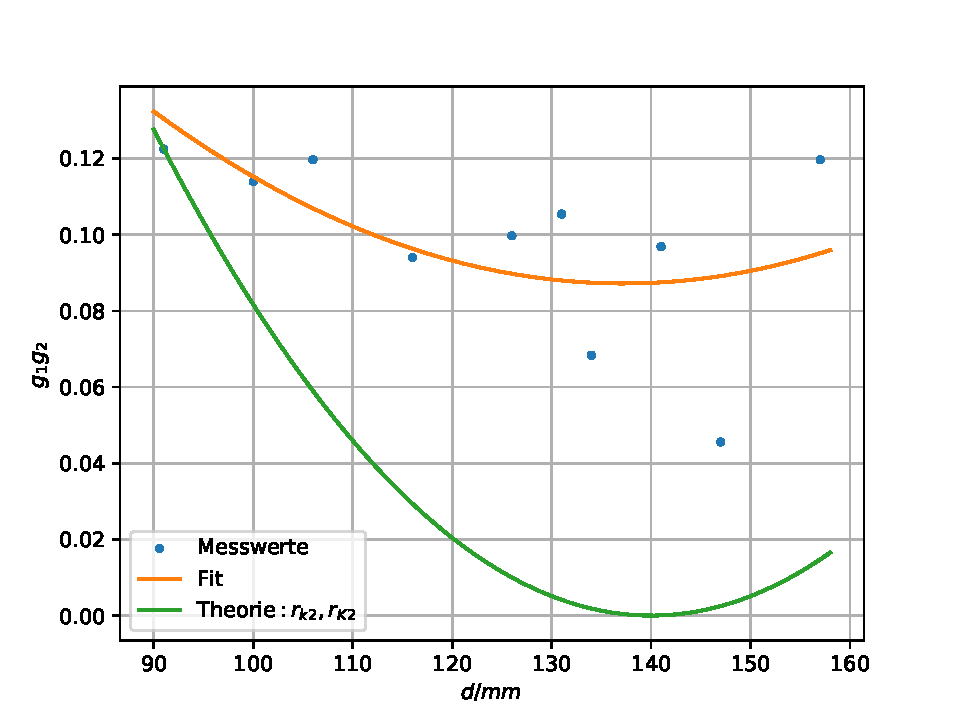
\includegraphics[width=0.8\textwidth]{../Messdaten/plots/konkon.pdf}
  \caption{Plot der in Tabelle \ref{tab: konkon} gelisteten Messwerte. Zusätzlich ist in der Grafik die bestimmte Ausgleichskurve und die Theoriekurve \eqref{} zu sehen.} %eqref
  \label{fig: konkon}
\end{figure}

\FloatBarrier
\FloatBarrier
\subsubsection{Konkav-Flache Konfiguration}
Die Messwerte sind in Tabelle \ref{tab: konflach} aufgelistet.
Eine Skalierung erfolgt mit dem Faktor $c=\num{0.46}$
\begin{table} 
\centering 
\caption{Aufgenommene Messwerte für die Untersuchung der Stabilitätsbedingung bei Konkav-Flache Konfiguration. Der Umskalierungsfaktor $c$ beträgt $\num{0.46}$.} 
\label{tab: konflach} 
\begin{tabular}{S S S } 
\toprule  
{$ d / \si{ \centi\meter}$} & {$ I_p / \si{ \milli\ampere}$} & {$ \frac{I_p\cdot c}{I_{p,max}}$} \\ 
\midrule  
75 & 0.15 & 0.46\\ 
82 & 0.13 & 0.40\\ 
87 & 0.11 & 0.34\\ 
94 & 0.10 & 0.31\\ 
99 & 0.09 & 0.28\\ 
106 & 0.00 & 0.00\\ 
\bottomrule 
\end{tabular} 
\end{table}

An die Messwerte wird eine Gerade
\begin{equation*}
  g(d)=md+a
\end{equation*}
gefittet. Die Parameter $m$ und $a$ werden mittels Regressionsberechnung zu
\begin{align}
  \label{eq: konflach}
  \begin{aligned}
    m&=\SI{1.29 \pm 0.29 e-2}{\per\milli\meter}\\
    a&=\num{1.46\pm0.27}.
  \end{aligned}
\end{align}
Die Regressionskurve wird mit den Messwerten und der Theoriekurve \eqref{} in Abbildung \ref{fig: konflach} dargestellt.

\begin{figure}[h!]
  \centering
  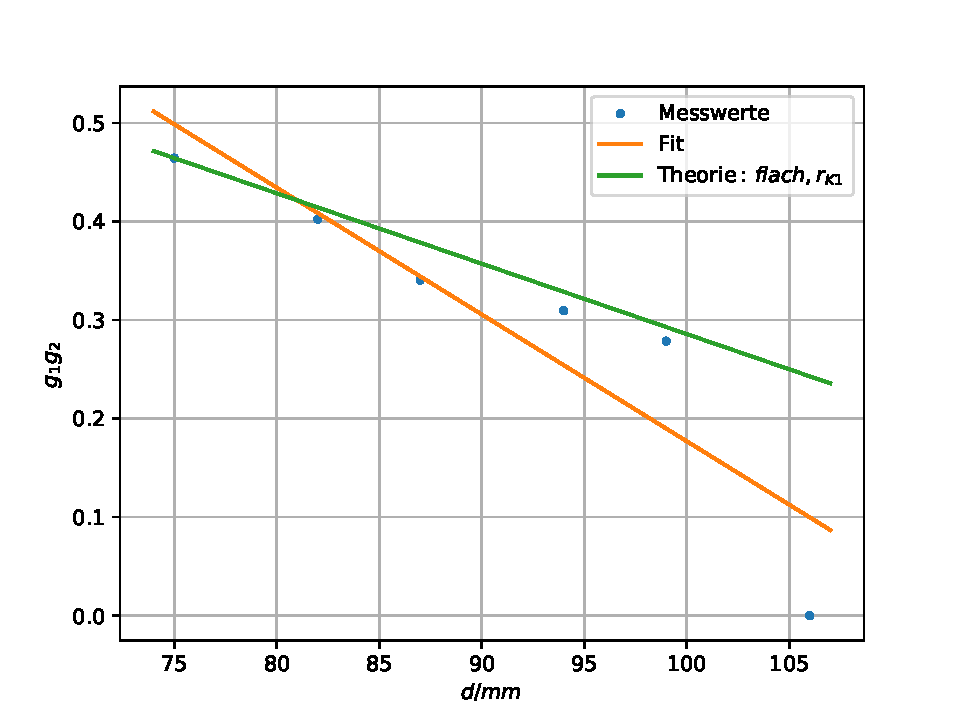
\includegraphics[width=0.8\textwidth]{../Messdaten/plots/konflach.pdf}
  \caption{Plot der in Tabelle \ref{tab: konflach} gelisteten Messwerte. Zusätzlich ist in der Grafik die bestimmte Ausgleichsgerade und die Theoriekurve \eqref{} zu sehen.}
  \label{fig: konflach}
\end{figure}
\FloatBarrier
